\chapter{Post Processing}
\label{chap:pp}

% Why post processing? Cool effects that can easily be applied to any
% project and reused.

In the previous sections geometry has been used to create the
landscape, sky and rendering it to the screen. Now we turn to screen
space effects, which do not rely on geometry, but will instead use the
final color image and the depth buffer to create the effects. Depth of
field, motion blur and a screenwide glow are all effects that can
easily be produced through post processing and there are many more.

% Easy to use important. Should handle most of the setup

We will try to create a general framework inside OpenEngine that can
handle most effects with the programmer having to do as little setup
as possible. It should also be possible to layer post processing
effects on top of each other, for example to combine a cel shader with
edge detection or optimizing blurring by using the separable
convolution technique.

\section{Structure}

In this section we will first outline the new scene node called
\class{PostProcessNode} and how it will help the programmer setup post
processing. Then we will discuss the specifics of rendering the scene,
applying the post process effect to it and how we eventually chose to
structure the rendering.

\subsection*{Post Process Node}

The \class{PostProcessNode} will apply a fragment program to
manipulate the image rendered while visiting subnodes in the scene
graph. Therefore it of course contains an \class{IShaderResourcePtr}
that points to the effect. It also contains a pointer to an OpenEngine
\class{FrameBuffer}, which the scene is rendered to. The postprocess
node also contains a \class{FrameBuffer}, where the final image can be
blitted into after the effect has been applied. This is useful for
some implementations of motion blur, that relies on the previous image
being availible.

In order to allow users of the PostProcessNode to focus on writing
their effects, the node will handle most of the setup as long as a few
naming conventions are followed. If a uniform named \textit{depth} is
detected then the subscenes depth texture will be bound to this
uniform. Similarly if \textit{imageN}, where \textit{N} is any
integer, is seen, then the \class{FrameBuffer}'s \textit{N}'th color
attachment will be bound to that uniform. The same goes for the final
image and the uniform name \textit{finalImageN}. The node can also
decide to improve performance by not blitting the final image, if this
isn't needed. Of course the previous image doesn't make sense in the
very first rendering, so when initialized the node binds the
not-processed scene image as the final image, and then after the first
frame it switches to the final image. And finally, if needed the node
will pass the time to the shader.

All of this has allowed us to cut back on doing setup and spend our
time writing cool and fun effects.

\subsection*{Rendering}

% render to a framebuffer

When the \class{RenderingView} visits the \class{PostProcessNode}, the
very first thing that needs to be done is storing the name of the
current render buffer and the viewports dimensions. These are needed
in order to restore them after the subscene has been rendered. With
the previous state saved, the \class{PostProcessNode}'s
\class{FrameBuffer} is bound and the subscene rendered to it.

\begin{lstlisting}[frame=,language=C++]
  GLint prevFbo;
  glGetIntegerv(GL_FRAMEBUFFER_BINDING_EXT, &prevFbo);
  Vector<4, GLint> prevDims;
  glGetIntegerv(GL_VIEWPORT, prevDims.ToArray());
  
  Vector<2, int> dims = node->GetDimension();
  glViewport(0, 0, dims[0], dims[1]);
  CHECK_FOR_GL_ERROR();
  glBindFramebufferEXT(GL_DRAW_FRAMEBUFFER_EXT, node->GetSceneFrameBuffer()->GetID());
  glClear(GL_COLOR_BUFFER_BIT | GL_DEPTH_BUFFER_BIT);
  CHECK_FOR_GL_ERROR();
  
  node->VisitSubNodes(*this);
\end{lstlisting}

% Apply the effect with depth testing set to always

When the scene has been rendered to the node's own
\class{FrameBuffer}, the previous framebuffer and viewport are
restored. The post process is then applied by binding the post process
effect and drawing a rectangle across the screen. To increase
performance the depth test is set to always allow all fragments.

\begin{lstlisting}[frame=,language=C++]
  glBindFramebufferEXT(GL_FRAMEBUFFER_EXT, prevFbo);
  glViewport(prevDims[0], prevDims[1], prevDims[2], prevDims[3]);
  
  // Gently disable the depth func (while preserving depth writes)
  glDepthFunc(GL_ALWAYS);
  // Then render the effect
  node->GetEffect()->ApplyShader();
  glRecti(-1,-1,1,1);
  node->GetEffect()->ReleaseShader();
  glDepthFunc(GL_LESS);
\end{lstlisting}

% Store the final image

If the post process effect relies on the final image from the previous
rendering, then now is the time to save the image. However recall from
earlier that the previous image was originally set in the effect as
the same as the current image. Therefore if this is the first
renderpass, the final image texture has to be bound to the effect, so
it is ready for use in the next pass. The final image can then be
blitted from the current renderbuffer into the renderbuffer that will
hold the final image.

\begin{lstlisting}[frame=,language=C++]
  FrameBuffer* finalFb = node->GetFinalFrameBuffer();
  if (finalFb != NULL){
    if (finalFb->GetID() == 0){
      // Initialize the final frame buffer and assign the
      // textures to the effect shader.
        ...
    }
    // Blit the images from the previous framebuffer to the final framebuffer
    glBindFramebufferEXT(GL_DRAW_FRAMEBUFFER_EXT, finalFb->GetID());
    glBlitFramebuffer(prevDims[0], prevDims[1], prevDims[2], prevDims[3], 
                      0, 0, dims[0], dims[1], 
                      GL_COLOR_BUFFER_BIT, GL_LINEAR);
    
    // Reset to previous fbo
    glBindFramebufferEXT(GL_FRAMEBUFFER_EXT, prevFbo);
  }
\end{lstlisting}

\section{Post Pocess Effect}

In this section we will take to a short look at some of the different
post process effects that we have created.

\subsection{Motion Blur}

While motion blurring may not be critical to outdoor environments,
many projects still benefit from it. Therefore one of the criteria
to the post process node was that it would allow an easy motion blur
implementation for existing and future open engine projects.

Motion blurring can be done in several ways. The simplest way
conceptually is to store the last $n$ images and then blend them
together. This creates a nice blurring effect across the last few
frames. The problem is that we then need to store the last few frames
in memory, giving us a memory overhead of 8-16 textures. Another
problem is that the blurring is framerate dependent, so low framerates
will make the blurring excessive, while high framerates will make it
non existent.

Another approach was proposed in GPU Gems 3, where the previous
ViewProjection matrix is used to calculate the previous position of a
fragment and then accumulate the colors between the current and
previous position. This approach however only creates blurring if the
camera is moved. A car that drives past the camera will crystal
clear. Another problem is that the shader becomes quite complex and
timeconsuming.

The algorithm that we settled on is a ghosting motion blur and
combines a low memory footprint with a fast shader. We use an
acuumulation texture for storing all the previous images blended
together, and then blend that together with the current image. That
way the effect from old images will tend toward 0 and the motion
blurring will produce nice looking blurred 'tails' on moving
objects. Ofcourse since we can only blur between rendered frames, a
fast turning camera will produce artefacts.

The result can be seen in \reffig{fig:dofMotionBlur}

\subsection{Glow}

When looking at natural outdoor environments in bright sunlight,
colors seem to blur or smeer together. We would like to reproduce this
effect using a fullscreen glow post process. 

Initally the effect was created in just a single shader. This shader
did ablur on the surrounding fragments and then blended that result
with the original fragment. This produced the results we where after,
but at a huge performance overhead. The problem was texture
lookups. To blur the surrounding fragments of an $N \times N$
rectangle, we required $N^2$ texture lookups. This performance problem
was solved by applying the separable convolution technique. In the
first post process pass a horizontal blurring is performed, then in
the second pass a vertical blurring is performed on the resulting
image of the previous pass and this is then blended together with the
original non-blurred scene. For an $N \times N$ rectangle we've now
reduced $N^2$ texture lookups to $2N$, while achieving the same
effect.

% @TODO show the non blurred + blurred = glow images

As can be seen on \reffig{fig:glow}, a subtle smeering gives a
smoother and more natural looking image. The shader that does the
vertical blurring can be seen in \reflst{lst:glowShader}.

% TODO ref appendix

%% \begin{listing}
%% \label{lst:glowShader}
%% \centering
%%   \lstinputlisting[language=C++]{../data/shaders/glow.frag}
%% \caption{The vertically blurring glow shader.}
%% \end{listing}


\subsection{Depth of field}

When filming or photografing through a lens an effect called depth of
field occurs. Essentially everything not in focus by the camera
becomes blurry, and the greater the difference between the object in
focus and the out-of-focus object the more blurry the object will
appear.

With the color texture and depth texture of the rendered scene it is
possible to emulate this effect. In our example the focus of the
camera will always be the center of the screen.

To create the effect we first have to determine how out of focus a
fragment is, which determines teh fragments blurring offset. This is
done by computing the difference between the depth at the center of
the screen and the depth at the fragment.

As before in the glow effect we again create the blur by sampling a
box around the fragment. This time though the distance between sample
points is not constant, but proportional to the blurring offset. The
fragments in focus or near focus have a small blurring offset and thus
won't be much blurred, while fragments with a high blurring offset
will be sampled inside a larger square and thus be blurrier.

Instead of doing a box blur, we decided to blur with a half circle
kernel, as can be seen on \reffig{fig:halfCircle}. To increase
effectivness we tried squaring the error term and came up with the
kernel in \reffig{fig:halfCircleSquared}, which while faster still
provided a pleasing result.

\begin{figure}
  \centering
  \subfloat[Half circle kernel.]{
    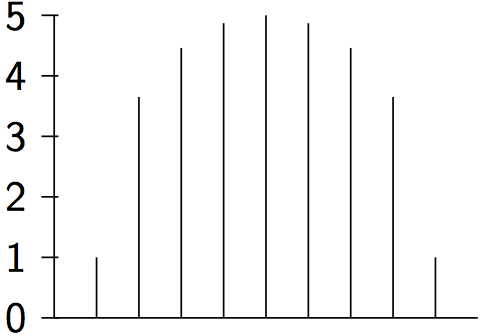
\includegraphics[width=6cm]{halfCircle}
    \label{fig:halfCircle}
  }
  \subfloat[Half circle kernel.]{
    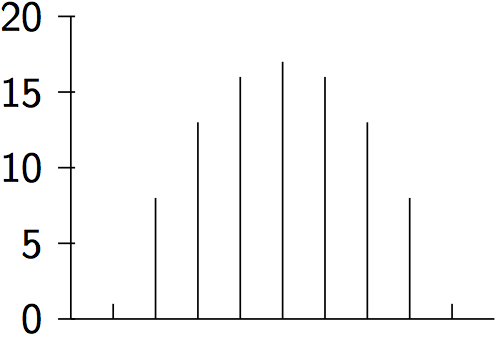
\includegraphics[width=6cm]{halfCircleSquared}
    \label{fig:halfCircleSquared}
  }
  \caption{Blurring kernels}
\end{figure}
%% \begin{figure}
%%   \label{fig:halfCircle}
%%   \centering
%%   \subfloat[Half circle kernel.]{
%%     \begin{minipage}{0.4\linewidth}
%%       \centering
%%       \begin{tikzpicture}[y=0.5cm, x=.35cm,font=\sffamily]
%%         %axis
%%         \draw (0,0) -- coordinate (x axis mid) (10,0);
%%         \draw (0,0) -- coordinate (y axis mid) (0,5);
%%         \foreach \y in {0,1,...,5}
%%         \draw (1pt,\y) -- (-3pt,\y) 
%%         node[anchor=east] {\y};
        
%%         \draw (1,0) -- coordinate (y axis mid) (1,1);
%%         \draw (2,0) -- coordinate (y axis mid) (2,3.65);
%%         \draw (3,0) -- coordinate (y axis mid) (3,4.46);
%%         \draw (4,0) -- coordinate (y axis mid) (4,4.87);
%%         \draw (5,0) -- coordinate (y axis mid) (5,5);
%%         \draw (6,0) -- coordinate (y axis mid) (6,4.87);
%%         \draw (7,0) -- coordinate (y axis mid) (7,4.46);
%%         \draw (8,0) -- coordinate (y axis mid) (8,3.65);
%%         \draw (9,0) -- coordinate (y axis mid) (9,1);
%%       \end{tikzpicture}
%%     \end{minipage}
%%   }

%%   \subfloat[Half circle squared kernel.]{
%%     \begin{minipage}{0.4\linewidth}
%%       \centering
%%     \begin{tikzpicture}[y=0.125cm, x=.35cm,font=\sffamily]
%%       %axis
%%       \draw (0,0) -- coordinate (x axis mid) (10,0);
%%       \draw (0,0) -- coordinate (y axis mid) (0,20);
%%       \foreach \y in {0,5,...,20}
%%       \draw (1pt,\y) -- (-3pt,\y) 
%%       node[anchor=east] {\y};
      
%%       \draw (1,0) -- coordinate (y axis mid) (1,1);
%%       \draw (2,0) -- coordinate (y axis mid) (2,8);
%%       \draw (3,0) -- coordinate (y axis mid) (3,13);
%%       \draw (4,0) -- coordinate (y axis mid) (4,16);
%%       \draw (5,0) -- coordinate (y axis mid) (5,17);
%%       \draw (6,0) -- coordinate (y axis mid) (6,16);
%%       \draw (7,0) -- coordinate (y axis mid) (7,13);
%%       \draw (8,0) -- coordinate (y axis mid) (8,8);
%%     \draw (9,0) -- coordinate (y axis mid) (9,1);
%%     \end{tikzpicture}
%%     \end{minipage}
%%   }
%% \end{figure}

The result can be seen on \reffig{fig:dofMotionBlur} where the hill in
the background and the horizon are slightly blurry. The shader that
creates the horizontal depth of field blurring can be seen in shader
HorizontalDepthOfField.frag.

\begin{figure}
  \label{fig:dofMotionBlur}
  \centering
  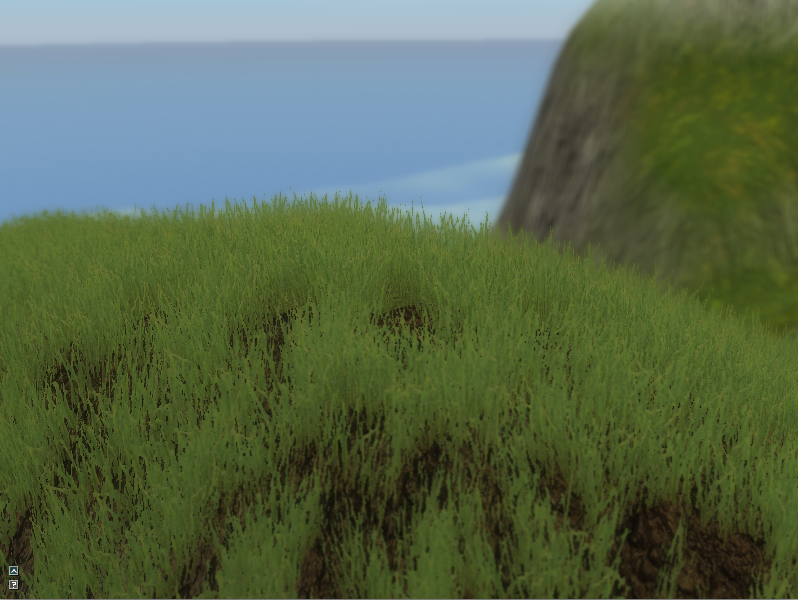
\includegraphics[width=7cm]{depthOfField}
  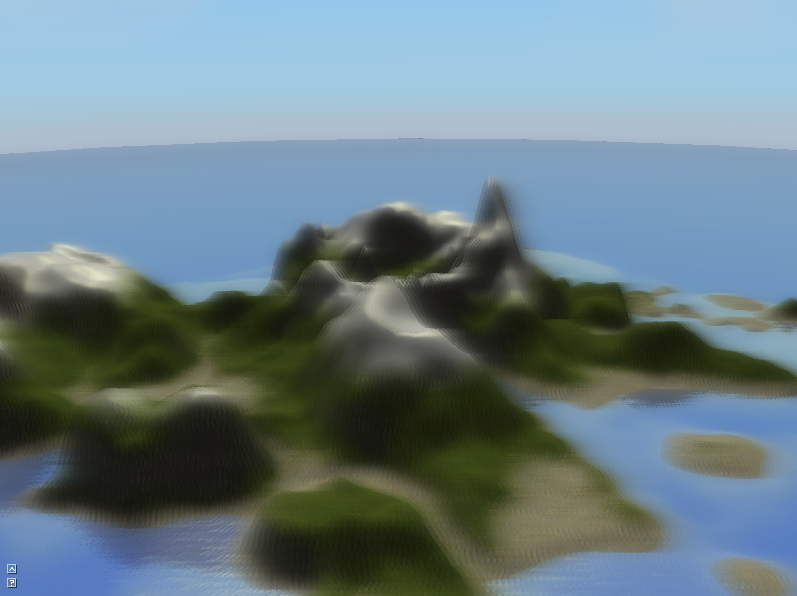
\includegraphics[width=7cm]{motionBlur}
  \caption{The left figure shows the depth of field effect with the
    focus on the front grass. The right image shows ghosting motion
    blur in action.}
\end{figure}



%%% Local Variables:
%%% mode: latex
%%% TeX-master: t
%%% TeX-PDF-mode: t
%%% End:
